\definecolor{meshOrange}{RGB}{238,145,0}
\definecolor{cellGreen}{RGB}{135,220,20}
\definecolor{eigenPurple}{RGB}{155,0,190}
\definecolor{axisGray}{RGB}{75,85,85}
\usetikzlibrary{arrows.meta}

\begin{figure}[H] 
\centering
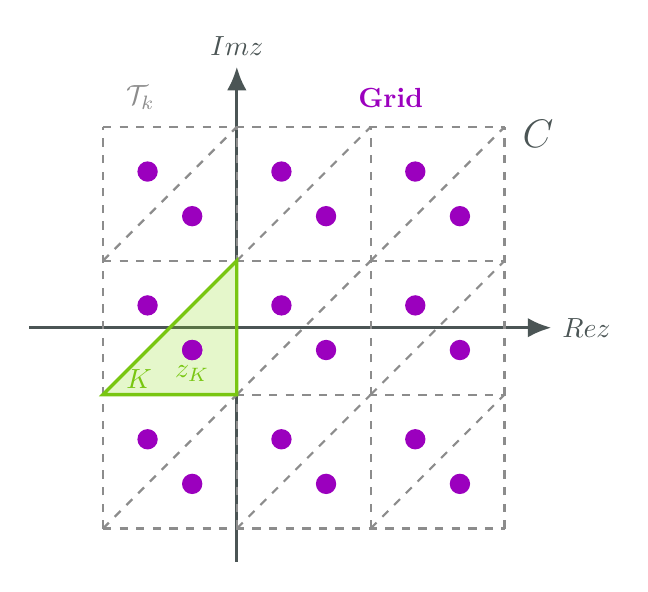
\begin{tikzpicture}[
    scale=1.7,
    axis/.style={
        axisGray,
        very thick,
        -{Latex[length=3mm,width=2.5mm]}
    },
    mesh/.style={
        gray!90,
        thick,
        dashed
    },
    selected cell/.style={
        cellGreen!90!black,
        very thick
    },
    barycentre/.style={
    circle,
    fill=eigenPurple,
    inner sep=2.6pt
    }
]

%------------------------------------------------
% Axes
%------------------------------------------------
\draw[axis] (-1.55,0) -- (2.35,0)
    node[right, axisGray] {$\operatorname{Re} z$};

\draw[axis] (0,-1.75) -- (0,1.95)
    node[above, axisGray] {$\operatorname{Im} z$};

\node[axisGray] at (2.25,1.45) {\Large $\mathbb{C}$};

%------------------------------------------------
% Highlighted triangular cell K
% Vertices: (-1,-0.5), (0,-0.5), (0,0.5)
%------------------------------------------------
\fill[cellGreen, opacity=0.22]
    (-1,-0.5) -- (0,-0.5) -- (0,0.5) -- cycle;

%------------------------------------------------
% Triangulation
%------------------------------------------------
\foreach \x in {-1,0,1,2}
    \draw[mesh] (\x,-1.5) -- (\x,1.5);

\foreach \y in {-1.5,-0.5,0.5,1.5}
    \draw[mesh] (-1,\y) -- (2,\y);

\foreach \x in {-1,0,1}{
    \foreach \y in {-1.5,-0.5,0.5}{
        \draw[mesh] (\x,\y) -- ++(1,1);
    }
}

\node[gray!90, font=\bfseries] at (-0.72,1.72) {$\mathcal{T}_k$};
%------------------------------------------------
% Barycentres of all triangles
%------------------------------------------------
\foreach \x in {-1,0,1}{
    \foreach \y in {-1.5,-0.5,0.5}{
        \node[barycentre] at ({\x+2/3},{\y+1/3}) {};
        \node[barycentre] at ({\x+1/3},{\y+2/3}) {};
    }
}

%------------------------------------------------
% Outline and label the selected cell K
%------------------------------------------------
\draw[selected cell]
    (-1,-0.5) -- (0,-0.5) -- (0,0.5) -- cycle;

\node[cellGreen!90!black, font=\bfseries]
    at (-0.73,-0.38) {$K$};

%------------------------------------------------
% Barycentre of selected cell and its label
% barycentre = (-1/3,-1/6)
%------------------------------------------------
\coordinate (zK) at (-0.333,-0.167);
\node[barycentre] at (zK) {};

% z_K label -- same orange as K
\node[cellGreen!90!black, font=\bfseries, below=2pt]
    at (zK) {$z_K$};

% \node[cellGreen, font=\bfseries, below=2pt]
%     at (zK) {$z_K$};

%------------------------------------------------
% Grid label
%------------------------------------------------
% \node[cellGreen, font=\bfseries]
%     at (1.15,1.18) {Grid};

% Grid label -- moved above the triangulation
% \node[cellGreen, font=\bfseries]
%     at (1.15,1.72) {Grid};
\node[eigenPurple, font=\bfseries]
    at (1.15,1.72) {Grid};



\end{tikzpicture}
% \vspace{-1em}
\caption[A Representative Triangulation of the Complex Plane]{A representative triangulation of the complex plane. As shown in purple, the collection of barycentres forms $\operatorname{Grid} \subset \mathbb{C}$ for Algorithm \ref{pseudospec}. As shown in green, each triangle is indexed by $K,$ with corresponding barycentre $z_K.$}
% \caption[A Representative Triangulation of the Complex Plane]{A representative triangulation of the complex plane.}
\label{Triang}
\end{figure} 

% \begin{figure}[H]
% \centering
% \begin{tikzpicture}[
%     scale=1.8,
%     axis/.style={
%         axisGray,
%         very thick,
%         -{Latex[length=3mm,width=2.5mm]}
%     },
%     mesh/.style={
%         meshOrange,
%         thick,
%         dashed
%     },
%     selected cell/.style={
%         cellGreen,
%         very thick
%     },
%     barycentre/.style={
%         circle,
%         fill=cellGreen,
%         inner sep=2.6pt
%     }
% ]

% %------------------------------------------------
% % Axes
% %------------------------------------------------
% \draw[axis] (-1.55,0) -- (2.35,0)
%     node[right] {$\operatorname{Re} z$};

% \draw[axis] (0,-1.75) -- (0,1.95)
%     node[above] {$\operatorname{Im} z$};

% \node[axisGray] at (2.25,1.45) {\Large $\mathbb{C}$};

% %------------------------------------------------
% % Highlighted triangular cell K
% % Vertices: (-1,-1/2), (0,-1/2), (0,1/2)
% %------------------------------------------------
% \fill[cellGreen,opacity=0.20]
%     (-1,-0.5) -- (0,-0.5) -- (0,0.5) -- cycle;

% %------------------------------------------------
% % Square grid
% %------------------------------------------------
% \foreach \x in {-1,0,1,2}
%     \draw[mesh] (\x,-1.5) -- (\x,1.5);

% \foreach \y in {-1.5,-0.5,0.5,1.5}
%     \draw[mesh] (-1,\y) -- (2,\y);

% % Diagonal subdivision of each square
% \foreach \x in {-1,0,1}{
%     \foreach \y in {-1.5,-0.5,0.5}{
%         \draw[mesh] (\x,\y) -- ++(1,1);
%     }
% }

% %------------------------------------------------
% % Barycentres of all triangles
% % Each square [\x,\x+1] x [\y,\y+1] is split into:
% % 1) (\x,\y), (\x+1,\y), (\x+1,\y+1)
% %    barycentre = (\x+2/3,\y+1/3)
% % 2) (\x,\y), (\x,\y+1), (\x+1,\y+1)
% %    barycentre = (\x+1/3,\y+2/3)
% %------------------------------------------------
% \foreach \x in {-1,0,1}{
%     \foreach \y in {-1.5,-0.5,0.5}{
%         \node[barycentre] at ({\x+2/3},{\y+1/3}) {};
%         \node[barycentre] at ({\x+1/3},{\y+2/3}) {};
%     }
% }

% %------------------------------------------------
% % Outline and label the selected cell K
% %------------------------------------------------
% \draw[selected cell]
%     (-1,-0.5) -- (0,-0.5) -- (0,0.5) -- cycle;

% \node[cellGreen!60!black,font=\bfseries]
%     at (-0.77,-0.38) {$K$};

% %------------------------------------------------
% % Label the barycentre z_K of the selected cell
% % barycentre of K = (-1/3,-1/6)
% %------------------------------------------------
% \node[barycentre] (zK) at (-0.333,-0.167) {};

% \node[
%     cellGreen!55!black,
%     font=\bfseries,
%     below right=1pt
% ] at (zK) {$z_K$};

% %------------------------------------------------
% % Label Grid
% %------------------------------------------------
% \node[cellGreen!60!black,font=\bfseries] at (1.45,1.15)
%     {$\operatorname{Grid}$};

% \draw[cellGreen!60!black,thick,->]
%     (1.15,1.02) -- (0.67,0.83);

% \end{tikzpicture}
% \end{figure}